\section{Zielsetzung}
\label{sec:ziel}
In diesem Versuch wird die magnetische Suszeptibilität paramagnetischer Stoffe bestimmt. Dies geschieht für drei verschiedene seltene Erden. Die Messung der dafür nötigen
Größen geschieht über eine Brückenschlatung.

\section{Theorie}
\label{sec:Theorie}

\subsection{Paramagnetismus}
\label{subsec:paramagnetismus}
Paramagnetismus ist eine eine Eigenschaft von Materie in einem Magnetfeld. Allerdings trifft diese Eigenschaft nicht auf jegliche Materie. Paramagnetische Stoffe haben ohne 
äußeres Magnetfeld keine eigene magnetische Ordnung. Außerdem ist bei solchen Stoffen das äußere Magnetfeld stärke als das innere. Daher werden paramagnetische Stoffe in ein
außen anliegendes Magentfeld hineingezogen. $\mu_{\text{r}}$ liegt bei paramagnetischen Stoffen $ < 1 $. Beispiele für paramagnetische Stoffe sind sogenannte 
\textit{seltene Erden}. Diese Stoffe werden in diesem Versuch verwendet. 

\subsection{Zusammenhang von Paramagnetismus und atomaren Drehimpuls}
\label{subsec:drehimpuls}
Damit Paramagnetismus auftreten kann, dürfen die Atome und Moleküle keine verschwindenden Drehimpulse haben. Wie in \autoref{subsec:paramagnetismus} bereits erwähnt, ist 
Paramagnetismus temperaturabhängig. Diese Abhängigkeit entsteht, wenn sich die magnetischen Momente der Moleküle ausrichten. Die magnetischen Momente sind mit den Drehimpulsen 
gekoppelt. Steigt nun die Temperatur eines paramagnetischen Stoffes, so steigt die kinetische Energie der Atome. Daher bewegen sich diese Stärker und stören so die Ausrichtung
der Momente. 

\subsection{Vom Drehimpuls zur Suszeptibilität}
\label{subsec:drehsus}
Es gibt drei Drehimpulse eines Teilchens die den Gesamtdrehimpuls festlegen. Der Banhdrehimpuls der Elektronenhülle, der Spin der Elektronen und Kerndrehimpuls. In schwachen 
Magnetfeldern hat der Kerndrehimpuls einen vernachlässigbar kleinen Effekt auf den Paramagnetismus. Der Gesamtdrehimpuls ergibt sich daher durch 
\begin{equation*}
    \vec{J} = \vec{L} + \vec{S}.
\end{equation*}
Dabei beschreiben $\vec{L}$ und $\vec{S}$ die Summe aller einzelnen Drehmomente der jeweiligen Teilchen. Durch die Quantenmechanik kann den Drehmomenten $\vec{L}$ und $\vec{S}$
ein magnetisches Moment zugeordnet werden. 
Die potentielle Energie der Einrichtungen der magnetischen Momente kann mittels des \textit{Landé-Faktors} $g_{\text{J}}$ und der Orientierungsquantenzahl $m$ durch 
\begin{equation}
    E_{\text{m}} = \mu_{\text{B}} g_{\text{J}} m
\end{equation} 
berechnet werden. Dabei ist $\mu_{\text{B}}$ das \textit{Bohrsche Mageton}. Nach Aufspaltung der Enrgieniveaus tritt der \textit{Zeeman-Effekt} auf. Um nun die Magnetisierung
berechnen zukönnen, muss die Häfugkeit bestimmter Orientierungen der magnetischen Moment herausgefunden werden. Diese verteilen sich gemäß der \textit{Boltzmann-Verteilung}
auf die  Energieunterniveaus. Nach Summation über die Enrgieniveaus kann ein mittleres magnetisches Moment berechnet werden. Diese lässt sich gemäß der \textit{Brillouin-Funktion}
berechnen. Diese Formel lässt sich allerdings im allgemeinen nicht analytisch lösen. Daher wird eine Näherung verwendet. Das Problem wird dabei in Raumtemperatur betrachtet und
es werden lediglich schwache Felder betrachtet. In dieser Näherung kann dann die Magnetisierung bestimmt werden.
\begin{equation*}
    M = \frac{1}{3}\mu_0 N g^2_{\text{J}} \mu^2_{\text{B}} \frac{J(J+1)B}{kT}
\end{equation*}
Daraus lässt sich dann gemäß Formel \eqref{eqn:Mchi} berechnen. 
\begin{equation}
    \label{eqn:chi1}
    \chi = \frac{1}{3}\mu_0 N g^2_{\text{J}} \mu^2_{\text{B}} \frac{J(J+1)}{kT}
\end{equation}   
Daraus folgt eine $\frac{1}{T}$-Abhängigkeit für $\chi$. Man nennt die Formel \eqref{eqn:chi1} \textit{Curiesches Gesetz}.

\subsection{Suszeptibilität paramagnetischer Substanzen}
\label{subsec:Berechnung}

Zunächst wird der Zusammenhang zwischen der Magnetfeldstärke $\vec{H}$ und der Suszeptibilität $\chi$ untersucht. Dabei hängt die Magnetfeldstärke $\vec{H}$ über 
\begin{equation*}
    \vec{B} = \mu_0 \vec{H}
\end{equation*}
zusammen. Dies gilt allerdings nur für ein homogenes Magnetfeld. Befindet sich Materie in einem Magnetfeld ändert sich der Zusammenhang um einen Summanden $\vec{M}$, welcher 
Magnetisierung gennant wird.
\begin{equation}
    \label{eqn:magnetfeld}
    \vec{B} = \mu_0 \vec{H} + \vec{M}
\end{equation}
Die Magnetisierung entsteht durch magnetische Momente der Atome in einer Substanz. Mittels der Suszeptibilität kann die Magnetisierung in Abhängigkeit von $\vec{H}$
ausgedrückt werden. 
\begin{equation}
    \label{eqn:Mchi}
    \vec{M} = \mu_0 \chi \vec{H}
\end{equation}
Hierbei besteht kein lineare zusammenhang zwischen $\vec{M}$ und $\vec{H}$, da $\chi$ sowohl von der Temperatur der Probe, sowie von $\vec{H}$ selbst abhängt.

\subsection{Suszeptibilität Selterner-Erd-Verbindungen}
\label{subsec:suzepseltenererden}
Ionen seltener Erden weisen einen starken Paramagnetismus auf. Wie in \autoref{subsec:drehimpuls} erklärt, folgt aus dieser Eigenschaft, dass die Elektronenhüllen dieser Stoffe
große Drehimpulse haben. Diese entstehen durch die 4f-Elektronen in der Elektronenhülle. 4f-Elektronen treten erst ab Ordnungszahlen $\geq 58$. Die 4f-Elektronen liegen weit
innerhalb der 6s-Schale, wodurch auch die Paramagnetische Eigenschaft seltener Erden erklärt werden kann. Mit den Hundschen Regeln kann der Gesamtdrehimpuls der 4f-Schale
bestimmt werden. Ist die Schale weniger als zur Hälfte gefüllt lässt sich der Gesamtdrehimpuls gemäß $\vec{J} = \vec{L} - \vec{S}$ berechnet werden. Ist die Schale dahingegen 
mehr als zur Hälfte gefüllt berechnet sich der Gesamtdrehimpuls nach $\vec{J} = \vec{L} - \vec{S}$. Dabei gilt Jeweils $\vec{L} = \sum \vec{s}_i$ und $\vec{S} = \sum \vec{l}_i$. 

\subsection{Beschreibung einer Messapparatur der Suszeptibilität}
\label{subsec:Messapparatur}
Für eine Messapparatur der Suszeptibilität ist es nötig ein Magnetfeld zu erzeugen. Dies geschieht häufig über eine Lange Spule, da das Magnetfeld im inneren der Spule sehr 
homogen ist. Um mit einer solchen Spule zu rechnen ist die Induktivität eine relevante Größe.
Für eine Spule in einem Vakuum gilt für die Induktivität die Formel $L = \mu_0 \frac{n^2}{l}F$. Dabei beschreibt $l$ die Länge der Spule und $F$ den Querschnitt der Spule.
Um die Suszeptibilität eines Materials zu bestimmen wird ein Stoff nun in das Magnetfeld der Spule eingeführt. Geschieht dies, so ändert sich die Induktivität der Spule. 
Da in der Realität eine Spule nicht vollständig mit einer Probe gefüllt wird, kann man die Formel der Induktivität anpassen.
\begin{equation}
    \label{eqn:L_M}
    L_{\text{M}} = \mu_0 \frac{n^2 Q}{l} + \chi \mu_0 \frac{n^2 Q}{l}
\end{equation} 
Da der Unterschied zwischen der gefüllten Spule und einer im Vakuum nur sehr gering ist, wir eine sehr hohe Auflösung für die Messung von $L$ benötigt,
um die Suszeptibilität zu bestimmen. Um die nötige Auflösung zu erreichen, können zwei möglichst identische Spulen verwendet werden. Dabei wird eine der beiden Spule nicht 
gefüllt und in die andere wird die Messprobe eingeführt. Die beiden Spulen werden über eine Brückenschaltung zusammengeschlossen. Mit einer solchen Schaltung, wie sie in
\autoref{fig:schaltplan} dargestellt ist, kann die Suszeptibilität nun über zwei Methoden bestimmt werden.
\begin{figure}
    \centering
    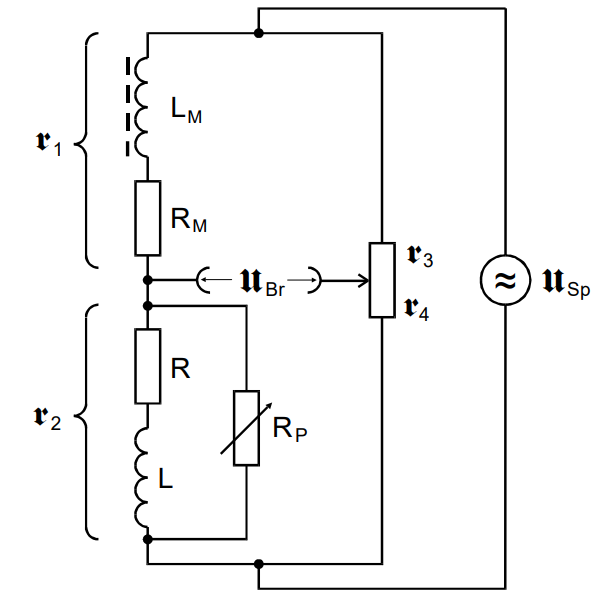
\includegraphics[width = .7\textwidth]{content/Schaltung1.PNG}
    \caption{Schaltplan einer Brückenschaltung zweier identischer Spulen. \cite{v606}}
    \label{fig:schaltplan}
\end{figure} 
Für die erste Methode müssen zunächst beide Spulen ohne Probe aufeinander abgestimmt werden. Dann wird die Brückenspannung gemessen, welche bei einführung der Probe in eine der 
Spulen entsteht. Aus der entstandenen Brückenspannung kann dann die Suszeptibilität berechnet werden.

Bei der zweiten Methode werden erneut beide Spulen aufeinander abgestimmt. Dann wird die Probe eingeführt und die beiden Brücken werden erneut aufeinander abgestimmt. Aus der
Änderung der Abgleichelemente kann nun die Suszeptibilität bestimmt werden.

Die Brückenspannung der ersten Methode kann aus Knoten- und Maschenregeln, sowie der Annahme, dass $\Delta L << L$, bestimmt werden. 
\begin{equation*}
    U_{\text{Br}} = \frac{\omega\mu_0\chi n^2Q}{4l}\frac{1}{\sqrt{R^2 + \omega^2\left(\mu_0\frac{n^2}{l}F\right)^2}}U_{\text{Sp}}
\end{equation*}
Um $\chi$ zu berechnen kann diese Formel nach $\chi$ umgestellt werden.
\begin{equation}
    \label{eqn:chi_theo}
    \chi = \frac{U_{\text{Br}}}{U_{\text{Sp}}}\frac{4l}{\omega\mu_0n^2Q}\sqrt{R^2 + \omega^2\left(\mu_0\frac{n^2}{l}F\right)^2}
\end{equation}
Dabei kann für hinreichend große Messfrequenzen $\chi$ angenähert werden.
\begin{equation}
    \label{eqn:chi:näherung}
    \chi = 4 \frac{F}{Q}\frac{U_{\text{Br}}}{U_{\text{Sp}}}
\end{equation}


Für die Bestimmung von $\chi$ über die zweite Methode wird die Abgleichbedingung $r_1R_4 = r_2R_3$ unter kleiner Abweichung $\Delta R$ betrachtet. Diese Abweichung entsteht
durch das Einführen der Probe in eine der Spulen. Die Abweichung $\Delta R$ lässt sich aus der Abgleichbedingung und der Näherung $\Delta L << L$ bestimmt.
\begin{equation*}
    \Delta R = \chi\frac{R_3}{2}\frac{Q}{F}
\end{equation*}
Damit folgt dann wieder eine Gleichung für $\chi$.
\begin{equation}
    \label{eqn:chimethode2}
    \chi = 2\frac{\Delta R}{R_3}\frac{F}{Q}
\end{equation}

\subsection{Unterdrückung von Störspannungen}
\label{subsec:unterdrückung}
Bei einer Schaltung, wie einer in \autoref{fig:schaltplan}, tritt das experimentelle Problem auf, dass Störspannungen an den Ausgangsklemmen die zu messende Brückenspannung
verdecken. Eine Lösung dieses Problem liegt in der Eigenschaft von monofrequenten Signalspannungen. Die Brückenspannung ist ebenfalls ein monofrequentes Signal. Daher kann man
durch einen \textit{Selektivverstärker}. Die Filterkurve eines Selektivverstärkers hat die Form eine gaußschen Glockenkurve. Ein Beispiel einer Filterkurve ist in \autoref{fig:Filterkurve}
zu sehen. Eine Filterkurve beschreibt die Abhängigkeit von
$\frac{U_{\text{A}}}{U_{\text{E}}}$ zur Frequenz $\nu$. Die Breite der Filterkurve ist ein Maß für die Spannungsunterdrückung. Damit im Zusammenhang steht die Güte $Q$. Die
Güte eines Selektivverstärkers kann gemäß
\begin{equation}
    \label{eqn:Guete}
    Q = \frac{\nu_0}{\nu_+ - \nu_-}
\end{equation}
berechnet werden. Dabei beschreibt $\nu_{\pm}$ die Frequenz bei welcher die Filterkurve $\frac{1}{\sqrt{2}}$ erreicht.

\begin{figure}
    \centering
    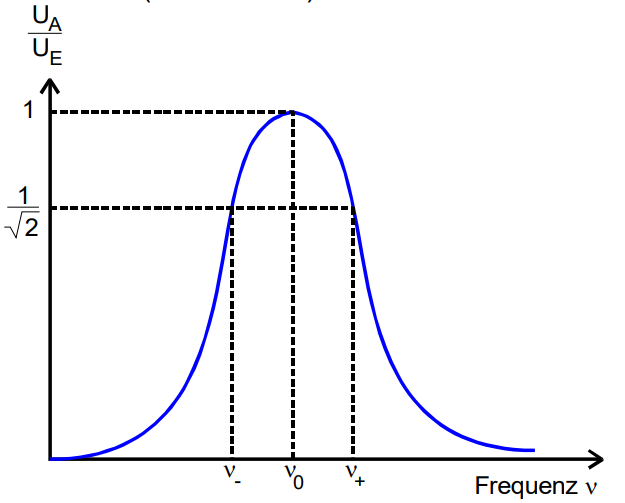
\includegraphics[width = .5\textwidth]{content/Filterkurve.PNG}
    \caption{Beispiel einer möglichen Filterkurve. \cite{v606}}
    \label{fig:Filterkurve}
\end{figure} 
